
\chapterbegin{Plan de entregas}

\minitoc


\section{Entregas}
\label{sec:planentregas}

El desarrollo de este proyecto estará dividido en una serie de entregas incrementales en las que se buscará crear un proyecto base ejecutable en un entorno de realidad virtual, al cual se le añadirán las distintas mecánicas del juego de manera gradual, obteniendo como resultado final tras la última entrega un videojuego completamente funcional y que cumpla los objetivos planteados para este trabajo de fin de grado.



\begin{itemize}
	\item{\textbf{Entrega 1}: Tener una escena en realidad virtual en la que un jugador pueda interactuar con el entorno usando avatares que representen sus manos.
		\begin{itemize}
			\item{Iteración 1: Crear un entorno funcional que sea capaz de ejecutarse de manera correcta en el dispositivo de VR de desarrollo.}
			\item{Iteración 2: Incorporar avatares de manos para el jugador. Añadir las posibles interacciones del jugador con sus manos: coger, soltar y lanzar objetos e intercambiar un objeto de una mano a la otra.}
			\item{Fecha de entrega estimada: 12 de mayo de 2023}
		\end{itemize}	
	}

	\item{\textbf{Entrega 2}: Diseñar e integrar en el proyecto las mecánicas y métodos necesarios para crear las pruebas de las que constará el juego.
		\begin{itemize}
			\item{Iteración 1: Diseñar las técnicas básicas que se usarán para evaluar las pruebas.}
			\item{Iteración 2: Crear en Unity las mecánicas básicas necesarias para realizar las distintas pruebas.}
			\item{Iteración 3: Poner a prueba la adaptación de varias personas al uso de la realidad virtual en general y en concreto a las mecánicas desarrolladas.}
			\item{Fecha de entrega estimada: 24 de junio de 2023}
		\end{itemize}	
	}
		
	\item{\textbf{Entrega 3}: Diseñar e incluir en el proyecto todos los escenarios y entornos necesarios para el juego.
	\begin{itemize}
		\item{Iteración 1: Diseñar los escenarios en los que se desarrolla en juego.}
		\item{Iteración 2: Creación e integración de los distintos escenarios y decorados para el proyecto.}
		\item{Iteración 3: Conocer la respuesta de varios usuarios ante los escenarios creados.}
		\item{Fecha de entrega estimada: 8 de julio de 2023}
	\end{itemize}	
	}

	\item{\textbf{Entrega 4}: Diseñar varias pruebas concretas de cada uno de los tipos y posteriormente añadirlas al proyecto.
	\begin{itemize}
		\item{Iteración 1: Diseñar todas las pruebas que habrá en el proyecto.}
		\item{Iteración 2: Implementación de 3 pruebas de cada tipo.}
		\item{Iteración 3: Evaluar la realización de las distintas pruebas por varios usuarios.}
		\item{Fecha de entrega estimada: 29 de julio de 2023}
	\end{itemize}	
	}

	\item{\textbf{Entrega 5}: Integrar todos los componentes para crear el flujo de juego y finalizar el proyecto.
	\begin{itemize}
		\item{Iteración 1: Unificar todo el desarrollo para crear la versión final jugable del proyecto.}
		\item{Iteración 2: Probar y evaluar las experiencias de varios jugadores en la versión completa del juego.}
		\item{Fecha de entrega estimada: 30 de agosto de 2023}
	\end{itemize}	
	}
	
\end{itemize}


%\begin{center}
%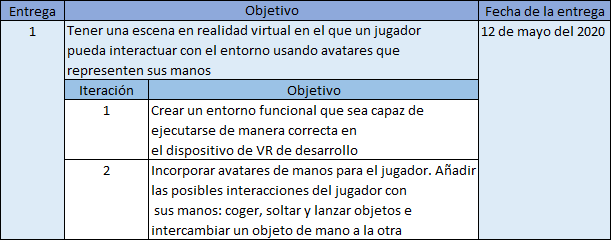
\includegraphics[width=1\textwidth]{03.EstudioProblema/05.PlanEntregas/00.Figuras/01.entrega_1.png}
%\end{center}

%\begin{center}
%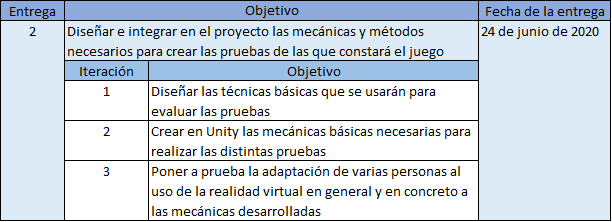
\includegraphics[width=1\textwidth]{03.EstudioProblema/05.PlanEntregas/00.Figuras/02.entrega_2.png}
%\end{center}

%\begin{center}
%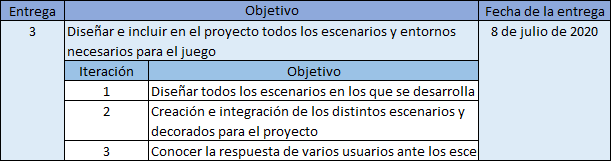
\includegraphics[width=1\textwidth]{03.EstudioProblema/05.PlanEntregas/00.Figuras/03.entrega_3.png}
%\end{center}

%\begin{center}
%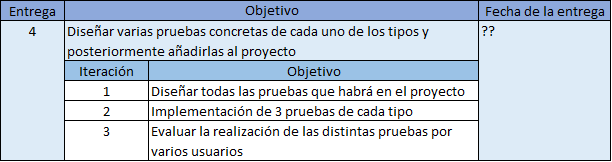
\includegraphics[width=1\textwidth]{03.EstudioProblema/05.PlanEntregas/00.Figuras/04.entrega_4.png}
%\end{center}

%\begin{center}
%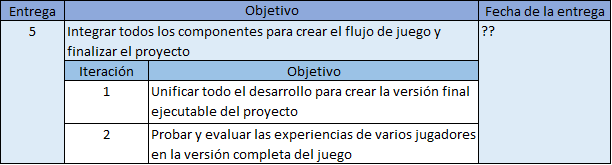
\includegraphics[width=1\textwidth]{03.EstudioProblema/05.PlanEntregas/00.Figuras/05.entrega_5.png}
%\end{center}

\chapterend